\paragraph{Dueling Deep Q-learning Network} The Dueling Deep Q-Learning Network \cite{wang2015dueling} explicitly separates the representation of state values and (state-dependent) action advantages. The dueling architecture consists of two streams that represent the value and advantage functions, which sharing a common convolutional feature learning module. The two streams are combined via a special aggregating layer to produce an estimate of the state-action function $Q$. This dueling network should be understood as a single $Q$ network with two streams that replaces the popular single-stream $Q$ network in existing algorithms such as DQN. The dueling network automatically produces separate estimates of the state value function and advantage function, without any extra supervision.
\begin{figure}[h]
\centering
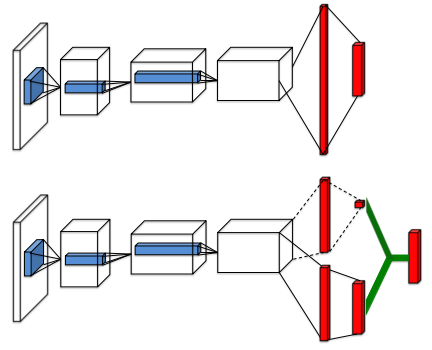
\includegraphics[width=5cm]{pic/dueling-architecture.PNG}
\caption{A popular single stream $Q$-network (\textbf{top}) and the dueling $Q$-network (\textbf{bottom}). The dueling network has two streams to separately estimate (scalar) state-value and the advantages for each action; the green output module implements equation (\ref{dueling_result}) to combine them. Both networks output $Q$-values for each action.} 

\end{figure}
\begin{equation} \label{dueling_result}
Q(s, a; \theta, \alpha, \beta) = V(s; \theta, \beta) + \left(A(s,a;\theta,\alpha) - \frac{1}{|\mathcal{A}|\sum_{a'}{}A(s,a^{'};\theta, \alpha)}\right)
\end{equation}
